% !TEX encoding = UTF-8 Unicode
\documentclass[parskip=full,11pt,twoside]{scrartcl}
\usepackage[utf8]{inputenc}

% section numbers in margins:
\renewcommand\sectionlinesformat[4]{\makebox[0pt][r]{#3}#4}

% header & footer
\usepackage{scrlayer-scrpage}
\lofoot{\today}
\refoot{\today}
\pagestyle{scrheadings}
\usepackage[T1]{fontenc}
\usepackage[sfdefault]{roboto}
\usepackage[german]{babel}
\usepackage[yyyymmdd]{datetime} % must be after babel
\renewcommand{\dateseparator}{-} % ISO8601 date format
\usepackage{hyperref}
\usepackage{amsmath} % for $\text{}$
\usepackage[nameinlink]{cleveref}
\crefname{figure}{Abb}{Abb}
\usepackage[section]{placeins}
%\usepackage{xcolor}
\usepackage[dvipsnames]{xcolor}
\usepackage{graphicx}
\usepackage{colortbl}
\usepackage{xcolor}
\usepackage[font=small,labelfont=bf]{caption} 
\usepackage{float}
\hypersetup{
pdftitle={Testbericht},
bookmarks=true,
}
\usepackage{csquotes}
\usepackage{upgreek}

\usepackage{ifthen}

\newcommand\urlpart[2]{$\underbrace{\text{\texttt{#1}}}_{\text{#2}}$}
\newcommand{\issueref}[1]{
    \href{https://git.scc.kit.edu/ap/Aurora/issues/#1}{(#1)}
}


% Titel GitLab issue number, Symptome, Grund, Behebung.
\newcommand{\regrtest}[5]{
    \subsection{#1 \issueref{#2}}
    \begin{itemize}
        \item \textbf{Symptom}
            #3
            %Hat man einen Term wie z.B. $\$plus\ 2\ 3\ \#\ foo$ eingegeben und klickt auf Step, so wurde der erste Schritt
            %fälschlicherweise als $\$plus\ 2\ 3\ foo$ ausgegeben.
        \item \textbf{Grund}
            #4
            %Javascript RegExp und die Java Regular Expression Bibliotheken unterscheiden sich in der Behandlung von dem
            %Regex-Shorthand \texttt{\textbackslash v}.
        \item \textbf{Behebung}
            #5
            %Der Regex-Shorthand wurde explizit ausgeschrieben so wie es vorgesehen war.
    \end{itemize}
}

\newcommand{\testline}[2]{
    \texttt{#1} & 
    \ifthenelse{\equal{#2}{Nicht getestet}}
        {\cellcolor{red!20}}
        {}
    \ifthenelse{\equal{#2}{Manuell getestet}}
        {\cellcolor{LimeGreen!20}}
        {}
    \ifthenelse{\equal{#2}{Automatisiert getestet}}
        {\cellcolor{green!20}}
        {}
    \ifthenelse{\equal{#2}{Nicht testbar}}
    {\cellcolor{gray!20}}
     {}
    #2 \\ \hline
}

\newcommand{\signed}[1]{%
   \unskip\hspace*{1em plus 1fill}%
   \nolinebreak[3]\hspace*{\fill}\mbox{\upshape #1}
}
 
\newenvironment{xquote}{%
   \begin{list}{}{%
     \rightmargin
     \leftmargin
   }
   \itshape
   \item[]
}
{\end{list}}

\begin{titlepage}
    \subject{Testbericht}
    \title{\textbf{$\uplambda$}urora}
    \subtitle{The Lambda Calculus IDE}


    \author{Iuliia Patrusheva, Alexander von Heyden\\
    Younis Bensalah, Max Nowak\\
    Nikolai Polley, Randy Seng}
\end{titlepage}


\begin{document}
\maketitle
\tableofcontents
\newpage

\begin{xquote}
    %Program testing can be a very effective way to show the presence of bugs, but is hopelessly inadequate for showing their absence.
    Testing shows the presence of bugs, not their absence.
    \newline
    \signed{-Edsger Wybe Dijkstra}
\end{xquote}

\section{Einleitung}
Trotz der Diversität heutiger Programmiersprachen teilen sich viele der damit geschriebenen Programme von Haus aus ein inhärentes Problem.
Setzt man sich nun das Ziel die Qualität, bzw. das Nutzererlebnis zu verbessern, ergeben sich für uns im Wesentlichen zwei Aufgabenbereiche.
\newline
Der eigentliche Schwerpunkt dieser Phase liegt darin, Aurora in einen möglichst stabilen Endzustand zu bringen.
Hierzu werden wir verschiedene Testkomponenten einsetzen, um jeweils bestimmte Teilfunktionen von Aurora testen zu können.
Die so gefundenen Fehler werden alle in diesem Dokument aufgelistet und dokumentiert.
\newline
Darüberhinaus kann eine Steigerung des Nutzererlebnisses auch durch das Erweitern der Funktionalität erreicht werden.
Teile des Funktionsumfangs, die nicht mehr in der Implementierungsphase umgesetzt werden konnten, können nun auch noch zu einem späteren Zeitpunkt zu Aurora hinzugefügt werden.

\subsection{JUnit/GWTTestCase}
Zeitgleich mit Beginn der Implementierung haben wir begonnen, zu unserem Code JUnit Testfälle zu schreiben.
Neben dem präventiven Schreiben von Testfällen, wurde auch zu jedem gefundenen Bug ein Test geschrieben, der genau diesen auslöste.
Nachdem der Fehler behoben wurde konnte so während der gesamten Implementierungs- und Qualitätssicherungsphase gewährleistet werden, dass ein einmal behobener Bug nicht erneut auftreten konnte.
Details, Ursachen, sowie die Behebung der Fehler sind in der Sektion \enquote{Regression Tests} festgehalten.

\subsection{GUI Tests}
Die GUI, als Schnittstelle zwischen dem Kern des Programmes und dem Nutzer, bedarf spezieller Testfälle zur Sicherstellung einer reibungslosen Interaktion.
Hierzu benutzen wir ein spezielles Framework, das bei jedem Aufruf einen Nutzer simuliert.
Dieser simulierte Nutzer kann, innerhalb von vordefinierten Abläufen, diverse Inputs, wie z.B. Tastatur- und Mausevents, an Aurora senden.
Somit können unterschiedlich komplexe Arbeitsabläufe automatisiert, und das Ergebnis mit einem vorher definiertem Zustand verglichen werden.



\section{Adaptionen des Pflichtenhefts}
\subsection{Musskriterien}

\subsubsection{Anzahl von dargestellten Schritten auswählen (M6)}
In Funktionaler Anforderung \textbf{5.1} wurde für dieses Musskriterium ein \enquote{3-Punkte-Button}
vorgestellt.
Alle Funktionalität des \enquote{3-Punkte-Button} wurde in den Step-Button integriert, da die zwei Buttons nahezu identisch waren. 

\subsection{Wunschkriterien}

\subsubsection{Ausgabe mit De Brujin-Indizes (K22)}
Es wird immer noch intern mit De Brujin-Indizes gerechnet, jedoch hat das Hinzufügen und Testen einer zusätzlichen Option,
die vom Benutzer verändert werden kann, zeitlich nicht gereicht.
Die Ausgabe erfolgt jetzt mit Variablennamen und es wird $\alpha$-Konversion durchgeführt.

\subsubsection{Benutzerdefinierte Auswahl (K10)}
Diese Auswertungsstrategie wurde wegen Zeitknappheit nicht implementiert.
Der Programmcode ist allerdings auf dieses Feature ausgelet und bietet
alle Methoden an, die für diese Strategie gebraucht werden.

%\subsection{Benutzerdefinierte Reduktionsstrategie (K10)}
% TODO kann gut sein, dass das noch implementiert wird.
% Das selbe gilt für:
% K5: Redexe highlighten.
% K16: Öffnen im neuen Tab.
% K20: Aurora Tutorial.
%TODO K16 neuer tab
%TODO HIGHLIGHTING K5
\subsubsection{Mobile Darstellung (K25)}
Eine explizite Anpassung der Graphischen Oberfläche an mobile Endgeräte wurde sehr früh in der Implementierung
ausgeschlossen.
Der Aufwand für den endgültigen Nutzen wäre zu groß gewesen, unter der Annahme das nicht viele Benutzter Lambda
Kalkül auf ihrem Smartphone programmieren.
Die Funktionalität des Programms ist auf einem modernen Smartphone dennoch gegeben.




\subsubsection{Pretty Print(K6)}
Wie bereits im Entwurfsdokument beschrieben ist kein Pretty Print implementiert.

\subsubsection{Standardbibliothek (K7)}
In der Beschreibung der Standardbibliothek wird die Aussage getroffen, dass
Churchzahlen in der Bibliothek sind.
Die Churchzahlen sind implementiert sind aber nicht in der Standardbibliothek,
da Funktionen in der Standardbibliothek namentlich in der Sidebar stehen und mit 
einem $\$$ vorangestellt werden müssen.
Beides ist nicht der Fall bei Churchzahlen

\subsubsection{Schleifenerkennung (K19)}
Wie bereits im Entwurfsdokument beschrieben ist dieses Wunschkriterium 
wegen zu geringen Nutzen nicht implementiert worden. 
Hiermit wird auch Nicht-Funktionale Anforderung \textbf{N10} nicht
mehr benötigt.

\subsubsection{Lokale Sessions (K23)}
Auch dies wurde wie im Entwurfsdokument beschrieben nicht implementiert.

\subsubsection{Tastatur-Shortcuts (K24)} \label{w:k24}

Der Run Button wird mit \enquote{ctrl + enter} ausgelöst
Da der Pause Button der Run Button ersetzt, wenn eine Reduktion ausgeführt wird,
ist auch der Shortcut des Pause Button \enquote{ctrl + enter}
Gleiches gilt für den Continue Button, der den Pause Button ersetzt.
Der Shortcut für Step ist \enquote{ctrl + space}
Resetted wird mit \enquote{ctrl + backspace}.

\subsection{Nichtfunktionale Anforderungen}

\subsubsection{Standardbibliothek und Benutzerbibliothek (N11) und (N22)}
Es gibt keine Beschränkung der Anzahl der Funktionen in den Bibliotheken
\subsubsection{Variablennamen (N17)}
Eine Variable darf groß oder kleingeschrieben werden, sie dürfen Zahlen
beinhalten, aber nicht als erstes Zeichen.
Das Sonderzeichen $\_ $ ist auch erlaubt worden, aber nicht als erstes Zeichen 
\subsubsection{Funktionsnamen (N18)}
Eine Funktion hat nun die gleichen Regeln wie eine Variable, sie muss aber 
weiterhin mit einem $\$$ beginnen.



\subsection{Testfälle}
Die Testfälle, die eine der vorher genannte Funktion referenzieren die adaptiert oder
gelöscht wurden.

%TODO T5.3 HIGHLIGHTING
%TOD T8 sharing und speichern
\subsubsection{Sprachenauswahl}
Der "ENG-Knopf" wurde durch einen Sprachenknopf ersetzt um sofort den Zweckes des Buttons
zu signalisieren.
\subsubsection{Teilen Funktion (T2)}
T2.1 beschreibt den Schrittmenüknop, der durch hovern erscheint. Da die Benutzbarkeit
des Programms durch unsichtbare Buttons erschwert würde, wurde sich für einen 
permanenten Button entschieden.
In T2.3 wird beschrieben, dass ein Popup mit einer Bestätigung erscheint.
Dies wurde geänder.
Der Share Latex Knopf öffnet ein unterschiedliches Popup.
Dieses Popup entählt den Latextext und zwei Buttons.
Der eine Button Kopiert den Text in die Zwischenablage, der andere
schließt das Popup.
Es wurde sich dafür entschieden, damit der Benutzer voher nochmal den
kopierten Text sieht und bei Bedarf nur Teile des Textes kopieren kann.

\subsubsection{Darstellung in Chrome (T3)}
In T3.3 wird erwähnt, dass der Nachtmodus durch den Button aktiviert werden muss.
Es wurde entschieden, dass der Nachtmodus der Default Modus ist und die Helle
Oberfläche durch den Button aktiviert wird.

In T4.3 wurde eine Bedingung gesetzt, dass die Ausgabe 4 ist, falls ein Wunschkriterium
erfüllt ist. Dieses ist erfüllt und die Ausgabe ist 4.

T4.4 Wie bereits erwähnt ist dieses Kriterium nicht implementiert.

\subsubsection{Testen von Highlighting (T5)}
T5.1 referenziert die Funktion plus.
Bei dem Schreiben des Tests wurde der schon damals definierte Beginn einer Funktion
vergessen und $\texttt{\$plus}$ gemeint. Diese Funktion ist unter dem Namen $\texttt{\$add} $ 
implementiert.

%todo correct highlightin%

\subsubsection{Testen der Standard- und Benutzerbibliotheken (T6)}
In Test T6.2 sollte die \enquote{first} Funktion in die Benutzerbibliothek
hinzugefügt werden. Da diese Funktion als wichtig gilt wurden sie bereits 
in die Standardbibliothek integriert. 
Die Tests funktionieren allerdings mit beliebigen anderen Funktionen.
Als neues Beispiel wird die Funktion threeissmaller der Benutzerbibliothek
hinzugefügt und mit Term $\$LEQ \ 3 \ 5$ gespeichert.

Der Benutzer kann nun in das Inputfeld $\texttt{\$threeissmaller} $ eingeben und 
im Ergebnis steht $\texttt{\$true}$
Mit dieser oder ähnlichen Modifikationen sind Tests T6.2 bis T6.4 ausführbar.


Erneut ist in T6.5 der Name der Funktion auf $\texttt{\$add}$ geändert worden.
T6.6 benutzt den Stepbutton und nicht den \enquote{3-Punkte-Button}.
Dies wird ab jetzt als bekannt vorausgesetzt und nicht erneut erwähnt.
Die Churchzahlen werden erst bei Bedarf in ihre wahren Terme überführt um die
Anschaulichkeit zu steigern. Damit sind die Schritte zu ausführlich.

Bei T6.7 ist im Pflichtenheft ein Fehler unterlaufen, anstelle des Run Buttons
war natürlich der Step Button gemeint
In T6.9 wurde minus durch $\texttt{\$sub}$ ersetzt. 

\subsubsection{Auswertungsstrategie und De Bruijn (T7)}
T7.2 Dass manuelle Drücken auf Redexe als Auswertungsstrategie wurde nicht implementiert.

\subsubsection{Sharing und Speichern (T8)}

% TODO T8.1 
% TODO t8.2
Die Funktion einen Term als Email zu verschicken, die in T8.3 getestet wird,
ist nicht implementiert.

T8.5 und T8.6 benutzen das Wunschkriterium History, welches in der Implementierung
ausgeschlossen wurde.
\subsubsection{Tutorial und Prettyprint (T9)}
T9.1 ein Zeilenumbruch wird erfolgen, er wird allerdings nicht intelligent erfolgen
wie im Test beschrieben.

\subsubsection{Ausgabe von Zwischenschritten (T10)}
In T10.2 wird gesagt, dass Zwischenschritte gelöscht wurde.
Es wurde sich dagen entschieden, da es eine schlechtere Benutzerfreundlichkeit
zur Folge gehabt hätte.

\subsubsection{Shortcuts}
Shortcuts werden wie in \ref{w:k24} beschrieben ausgelöst.


\section{Regression Tests}
Regression Tests sollen verhindern, dass Modifikationen an der Software, die unter anderem durch Wartung oder Korrektur von Komponenten entstehen kann, nicht dazu führen,
dass ehemals behobene Fehler erneut auftreten.
Um diesen Ansprüchen gerecht zu werden, ist es zwingend erforderlich, dass so früh wie möglich damit begonnen wird Testfälle zu schreiben,
weswegen wir bereits während der Implementierungsphase damit begonnen haben, Testfälle zu entwerfen, um die Korrektheit von Aurora zu gewährleisten.
Im folgenden, werden Bugs vorgestellt, die uns im Laufe der Implementierung bzw. Qualitätssicherung aufgefallen sind.
Die Fehler werden beschrieben, die Symptomatik festgehalten und die Behebung annotiert.
Vor der Behebung eines Fehlers, musste ein Regression Test geschrieben werden, der ebendiesen auslöste, nachdem der Fehler behoben wurde, durfte er dementsprechend nicht mehr ausschlagen.
Bugs wurden durchgehend in einem Issue Tracker festgehalten, sobald eine Issue geschlossen werden konnte, wurde der commit vermerkt, der den Fehler behoben hat.


\regrtest{Schrittzahl im Schrittfenster fängt mit falschen Index an}{120}{
	Wir stellen die Schrittzahl auf 2 ein.
	Es wird ($\lambda$x. x x)($\lambda$x. x x) in den Code-Editor eingegeben,
	dann auf den Run Button klickt, dann ein paar Sekunden gewartet und auf den Pause-Button geklickt.
	Es werden 2 Schritte im Schrittfenster angezeigt.
	Beispielsweise tragen diese die Nummern 101 und 102.
	Klickt man nun auf den Step Button, dann werden die 2 Schritte, die ausgegeben werden, die Nummern 104 und 105.
	Dabei wird die Nummer 103 ausgelassen.
}{
Der EditorPresenter übergibt der EditorView via dem EditorDisplay den falschen Schrittindex.
Der EditorPresenter hat bei der Berechnung des Schrittindex einen falschen Offset angegeben, welcher zum Fehler führt.
}{
Es wird beim EditorPresenter der richtige Offset zur Berechnung des Schrittindex angegeben.
}

\regrtest{Leerer Input in StepNumber TextBox führt zu nicht valide, dargestellten Wert}{133}{
	Lösche den gesamten Input in StepNumber TextBox, so dass diese leer ist. Klicke auf eine beliebige Stelle in der Aurora WebApp.
	Klicke zum Beispiel auf den Input Editor, so dass die StepNumber TextBox den Fokus verliert.
	Die StepNumber TextBox bleibt leer, obwohl sie eigentlich eine valide Schrittzahl anzeigen sollte.
}{
Die StepNumber TextBox überprüft den Input nach jeder neuen Eingabe.
Falls diese nicht valide ist, wird der letzte valide Wert angenommen.
Zudem wird auch eine leere TextBox akzeptiert, da auch valide Werte der Länge 1 eingegeben werden sollen.
Wenn die TextBox leer ist und den Fokus verliert, dann wird nicht der letzte valide Wert angenommen, da kein BlurHandler der StepNumber Textbox registriert wurde,
der den Wert wieder auf den letzten validen Wert setzt.
}{
Der StepNumber TextBox wird ein BlurHandler hinzugefügt, der den letzten validen Wert der StepNumber TextBox zuweist.
}

\regrtest{Das Ausführen einer nicht definierten Bibliotheksfunktion sollte einen Fehler anzeigen}{143}{
	Man gibt einen regulären $\lambda$-Term ein, der eine nicht definierte Bibliotheksfunktion enthält, ein und drückt auf den Run Button.
	Es wird keine Fehlermeldung angezeigt.
}{
Das Anzeigen von Fehlern, bei Eingabe eines ungültigen $\lambda$-Terms, wurde noch nicht implementiert.
}{
Implementiere die Funktionen displaySemanticError und displaySyntaxError in der Klasse EditorView.
Bei Ausführen der Berechnung eines ungültigen $\lambda$-Terms sollte in ein Zustandsübergang von RunningState auf DefaultState erfolgen.
Deswegen wird jedem Zustand eine neue Kante errorDisplayed hinzugefügt und implementiert.
}

\regrtest{Kommentare mitgeparst}{151}{
	Hat man einen Term wie z.B. $\$plus\ 2\ 3\ \#\ foo$ eingegeben und klickt auf Step, so wurde der erste Schritt fälschlicherweise als $\$plus\ 2\ 3\ foo$ ausgegeben.
}{
Javascript RegExp und die Java Regular Expression Bibliotheken unterscheiden sich in der Behandlung von dem Regex-Shorthand \texttt{\textbackslash v}.
}{
Der Regex-Shorthand wurde explizit ausgeschrieben so wie es vorgesehen war.
}

\regrtest{Hinzufügen einer benutzerdefinierten Bibliotheksfunktion soll in allen Zuständen der View außer RunningState möglich sein}{172}{
	Gibt man einen gültigen $\lambda$-Term in das Feld ein und klickt auf den Run Button.
	Dann ist das Hinzufügen einer benutzerdefinierte Bibliotheksfunktion nicht möglich.
}{
Der SidebarView wird mitgeteilt, dass nur in den Zuständen DefaultState und
FinishedFinishedState das Hinzufügen von benutzerdefinierten Bibliotheksfunktionen möglich ist.
}{
Wir erlauben das Betätigen des AddFunctionButton in allen Zuständen außer RunningState,
indem wir auf den AddFunctionButton die Methode setEnabled(true) aufrufen.
}

\regrtest{Ungültige Funktionsnamen bewirken Exception}{179}{
	Stand: Dialog zum Hinzufügen von einer neuen Benutzerbibliotheksfunktion is offen.
	Gibt man einen ungültigen Namen ein und drückt auf Add, schließt sich der Dialog und die Funktion wird nicht hinzugefügt.
	Auch sieht man eine UmbrellaException in der JavaScript Konsole.
}{
Der Fehler ist klassisch. Es wurde vergessen, den Rückgabewert von \texttt{RegExp.exec(..)} auf \texttt{null} zu überprüfen.
}{
Der mögliche \texttt{null}-return wird abgefangen und jetzt richtig behandelt.
}

\regrtest{Reduktion mit einer Libraryfunktion schlägt fehl}{172}{
	Als die Funktion $\$$infinity mit dem Term ($\lambda$x. x x)($\lambda$x. x x) der
	Benutzerbibliothek hinzugefügt wurde und sie in
	das Eingabefeld geschrieben wurde, wurde der Term nicht reduziert.
}{
Die Strategie baut einen Redexpath, der auf eine Applikation zeigt.
Als die Applikation aber in einer Funktion war, wurde sie nicht gefunden und es wurde ein Error geworfen.
Bei der Entwicklung des Betareduzierers wurde vernachlässigt, dass es auch Redexe in Funktionen geben kann.
Die meisten Funktionen sind zwar nicht mit sich selbst reduzierbar, da man sonst die Funktion zuerst reduzieren würde und dann hinzufügen würde.
Dennoch muss es möglich sein auch Funktionen nicht in Normalform hinzuzufügen.
}{
Wenn der Redexpath entlanggegangen wird und er auf eine Funktion zeigt, wird diese in ihren Term umgewandelt und dann wird dieser Term abgestiegen.
}

\regrtest{Alphakonversion ist nicht korrekt}{134}{
	Als 2 2 in das Inputfeld gegeben wurde und der Simplifier noch nicht implementiert war, wurde im Resultfeld das Ergebnis:
	$\lambda$z.$\lambda$z.z1(z1(z1(z1 z)) angezeigt.
	Intern war die Berechnung zwar korrekt und die Churchzahl 4 war berechnet worden,
	aber die Alphakonversion war inkorrekt, da festgelegt wurde, dass jede Variable, der eine Nummer angehängt wurde,
	eine freie Variable und keine gebundene Variable ist.
}{
Zu diesem Zeitpunk lief Alphakonversion folgendermaßen ab.
Jede Abstraktion suchte nach freien Variablen, die den gleichen Namen wie die Abstraktion hatten.
Falls dies der Fall war, wurde der freien Variable eine 1 angefügt.
Bei der Suche nach den freien Variablen wurde gleichzeitig jede gebundene Variable, die auf die Abstraktion zeigt,
mit einer freien Variable mit dem Namen der Abstraktion ersetzt.
Das Ergebnis ohne Alphakonversion wäre in Debruijnindizes:
$\lambda$z. $\lambda$z. 2 (2(2(2 1))).

Nach diesem ersten Schritt wäre es $\lambda$z. $\lambda$z. z(z(z(z 1))) wobei die $z$ freie Variablen wären und nicht mehr gebundene Variablen.
Vergessen wurde, dass es möglich ist, dass eine Abstraktion eine andere Abstraktion mit selben Namen im Body hat.
Jetzt wurden bei der zweiten Abstraktion erkannt, dass die freien Variablen den gleichen Namen wie die zweite Abstraktion haben,
und dann wurden sie alle alphakonvertiert zu z1 was dem Nutzer gesagt hätte, dass dies freie Variablen wären.
Durch die gebundene Variable $z$ am Schluss ist ein weiteres Problem aufgefallen:
Wie lassen sich diese  zwei unterschiedliche Ausdrücke noch in Debruijndarstellung mit Alphakonversion kenntlich machen.
$\lambda x.\lambda x. 1$
$\lambda x. \lambda x. 2$
Dies wurde zu diesem Zeitpunkt noch nicht berücksichtigt.
}{
Da dieses erste Problem dadurch herrührte, das die gebundenen Variablen gleichzeitig mit der Suche nach den freien Variablen passierte,
wurde dies in einen extra Schritt verfrachtet.
Es wurden zuerst freie Variablen auf Alphakonversion überprüft und erst dann die gebundenen Variablen ersetzt.
Um das zweite Problem zu beheben, wurde ein Visitor vor die Suche nach den freien Variablen gesetzt, der Namen von Abstraktionen ändert,
sollten sie gleich heißen wie eine Abstraktion in deren Body sie sind.
Dies führte zu einer funktionellen Alphakonversion, allerdings wurde uns mitgeteilt, dass man nicht den Namen von freien Variablen ändern sollte.
Sollte eine freie Variable mit gleichen Namen gefunden werden, muss der Name der Abstraktion geändert werden, nicht der Name der freien Variable.

Dies führt final zu folgender Struktur:
Es gibt einen Visitor, der den Term traversiert und bei jeder Abstraktion folgende Aktionen ausführt:
Er initialisiert einen weiteren Visitor, der den Term traversiert und nach Abstraktionen sucht, die den gleichen Namen haben wie die Abstraktion,
von der der Visitor gestartet ist.
Falls eine gefunden wurde, wird der Name dieser zweiten Abstraktion eine Zahl angehängt.

Als Beispiel: $\lambda z. \lambda z. \lambda z. ...$ wird zu $\lambda z. \lambda z1. \lambda z1. ...$
und wenn der ursprüngliche Visitor zu der zweiten Abstraktion kommt, wird daraus $\lambda z. \lambda z1. \lambda z2. ...$.
Dann wird nach freien Variablen gesucht, die den gleichen Namen haben wie die ursprüngliche Abstraktion.
Falls dies der Fall ist, wird der ursprünglichen Abstraktion ein $\_ alpha$ hinzugefügt.
In dem Beispiel $\lambda z. z$, bei dem das zweite $z$ eine freie Variable ist, wird dies zu $\lambda z \_ alpha. \  z$ verändert.
Hier wird keine Zahl an die Abstraktion gehängt, um dem Benutzer, klar zu machen, welche Form von Alphakonversion stattgefunden hat.
Wenn der Name der Abstraktion geändert wird, muss  nach neuen freien Variablen gesucht werden, die den gleichen Namen wie die neue Abstraktion haben.
Es könnte vorkommen, dass ein Tester diesen folgenden Term auf Alphakonversion testet:
$\lambda z. z \ z\_ alpha$ wobei $z$ und $z\_ alpha$ freie Variablen sind.
Hier wäre nach nur einem Schritt $z\_ alpha$ als gebundene Variable zu erkennen und nicht als freie Variable.
Deswegen muss erneut nach freien Variablen gesucht werden die den gleichen Namen besitzen.
In diesem Sonderfall würde erneut ein $\_ alpha$ an den Abstraktionsnamen angehängt werden.

Wenn dies vollbracht ist, werden gebundene Variablen durch freie Variablen mit dem Namen der Abstraktion ersetzt.
}

\regrtest{ShareLateX Ausgabe kompiliert nicht in Latex}{171}
{
	Texte, die von dem Share Latex Button kopiert wurden, kompilierte nicht in Latex
}{
Die Math Umgebung wurde nicht korrekt geschlossen und nicht alle Sonderzeichen wurden abgefangen.
}{
Die Methode wurde so restrukturiert, damit der Latextext komplett in der Math Umgebung residiert und
bei Notwendigkeit von anderen Textarten $\backslash$texttt$\{ \}$  und $\backslash$texttt$\{ \}$
verwendet werden.
}

\regrtest{Funktion wird nicht mit Funktionsname dargestellt, obwohl sie nicht reduziert wurde}{200}
{
	Die Eingabe $\lambda x. \$ \texttt{true}$ ist nicht reduzierbar und sollte nicht verändert werden.
	Dennoch wird im Ausgabefeld $\lambda x. \lambda t. \lambda f. t$ ausgegeben.
}{
Der Visitor, der nach gebundenen Variablen sucht, traversiert auch in die Funktion.
Bei der Implementierung wurde ignoriert, dass es unmöglich ist, dass eine Funktion eine gebundene Variable besitzt,
die nach außerhalb der Funktion zeigt.
}{
Bei der Suche nach gebundenen Variablen wird nicht mehr durch Funktionen traversiert sondern nur der Name
der Funktion zurückgegeben.
Damit wird nicht mehr nach nicht vorhandenen gebundenen Variablen gesucht und der Name der Funktion wird 
immer angezeigt, wenn sie nicht verändert wurde.
}


\section{Testfallszenarien}
Zu Beginn unseres PSE Projektes haben wir uns mehrere Testfallszenarien ausgedacht, und im Pflichtenheft festgehalten.
Jedes dieser Szenarien deckt für sich einen kleinen Teil der Funktionalität von Aurora ab, nacheinander ausgeführt ergänzen sie sich jedoch gegenseitig und decken einen großen Teil der nach außen sichtbaren Funktionen ab.
Im folgenden ist eine Auflistung aller Testfallszenarien zu finden, die mit der finalen Version von Aurora funktionieren werden.
Testfallszenarien, die auf Funktionen basieren, welche nicht Teil der finalen Version sein werden, sind, um Verwirrungen zu vermeiden, in der folgenden Auflistung nicht vorhanden.
\newline
\textbf{Oder doch oder was oder wie???}




\subsection{Testabstufungen}
Funktionalität innerhalb eines Programmes unterscheidet sich in vielerlei Hinsicht.
Demzufolge schwierig gestaltet es sich, für alle Funktionen gleichermaßen automatisierte Testfälle zu entwerfen.
Während es uns im Backend gelungen ist, eine fast flächendeckende Überdeckung zu erzielen, hat es sich, insbedondere in Teilen des Presenters und des Frontends, als wesentlich schwieriger erwiesen, eine ähnlich gute Abdeckung zu erreichen.
Zur besseren Darstellung unserer Tests haben wir uns dazu entschieden, nicht nur zwischen \enquote{automatisiert}, und \enquote{nicht} getestet zu unterscheiden, sondern auch Graustufen einzuführen, die sich dazwischen befinden.

\subsubsection{Nicht getestet}
Für nicht getestete Funktionen existieren keinerlei Tests jeglicher Art.
Sie wurden auch während der Entwicklung nicht regelmäßig von Hand ausprobiert.

\subsubsection{Von Hand getestet}
In bestimmten Szenarien war das Schreiben von komplett automatisierten Testfällen wesentlich aufwendiger als in anderen.
Falls es sich in gegebenem Szenario um Funktionen gehandelt hat die teilweise schon von anderen Tests überdeckt wurde,
    bzw. um Funktionen, die ggf. durch das Drücken eine Knopfes erneut ausgelöst werden konnten, haben wir und in bestimmten Fällen dazu entschieden,
    diese Szenarien in regelmäßigen Abständen von Hand zu testen.

\subsubsection{Automatisierte Tests}
Die meisten unserer Testfälle erfolgen automatisiert.
Hierzu zählen sowohl White, als auch Black-Box-Tests, die regelmäßig und automatisiert ausgeführt werden.
Insbesondere werden diese Testfälle auch von GitLab, nach jedem push, in einen beliebigen branch ausgeführt.

\subsection{Tests}

\subsubsection{Sprachenauswahl}
    Getestet:
    Sprache ist auswählbar (F37)

    \label{shortcuts}
    \begin{center}
        \begin{tabular}{ p{9cm} p{4cm}}
            Testfall & Testgüte \\ \hline
            \testline{T1.1}{Manuell getestet}
            \testline{T1.2}{Manuell getestet}
        \end{tabular}
    \end{center}

\subsubsection{Teilen-Funktion}
    Getestet:
    LaTeX-Export (F55)

    \label{shortcuts}
    \begin{center}
        \begin{tabular}{ p{9cm} p{4cm}}
            Testfall & Testgüte \\ \hline
            \testline{T2.1}{Manuell getestet}
            \testline{T2.2}{Manuell getestet}
            \testline{T2.3}{Automatisiert getestet}
        \end{tabular}
    \end{center}

\subsubsection{Darstellung in Chrome}
    Getestet:
    Korrekte Darstellung in Google Chrome (N1),
    Eingabefeld (F1),
    Zeilennummern (F2),
    Night Mode (F38),
    Mobile Darstellung (F39)

    \label{shortcuts}
    \begin{center}
        \begin{tabular}{ p{9cm} p{4cm}}
            Testfall & Testgüte \\ \hline
            \testline{T3.1}{Manuell getestet}
            \testline{T3.2}{Manuell getestet}
            \testline{T3.3}{Manuell getestet}
        \end{tabular}
    \end{center}

\subsubsection{Eingabe und korrektes Ergebnis}
    Getestet:
    Eingabefeld (F1),
    Zeilennummern (F2),
    Eingabefeld bearbeiten (F3),
    Autovervollständigung von Klammern (F4),
    Keine Änderungen während der Auswertung (F6),
    Schleifenerkennung (F42),
    Kein Timeout (F43),
    Run (F14),
    Normalreihenfolge (F27),
    $\beta$-Reduktion (F40),
    Auswertung beendet (F41),
    Ausgabefeld (F32),
    Reset (F16),
    Pause (F17),
    Continue (F18),
    Ausgabefeld nicht editierbar (F33),
    Kommentare (F8)

    \label{shortcuts}
    \begin{center}
        \begin{tabular}{ p{9cm} p{4cm}}
            Testfall & Testgüte \\ \hline
            \testline{T4.1}{Automatisiert getestet}
            \testline{T4.2}{Automatisiert getestet}
            \testline{T4.3}{Automatisiert getestet}
            \testline{T4.4}{Nicht testbar}
            \testline{T4.5}{Automatisiert getestet}
            \testline{T4.6}{Automatisiert getestet}
            \testline{T4.7}{Automatisiert getestet}
            \testline{T4.8}{Automatisiert getestet}
            \testline{T4.9}{Automatisiert getestet}
            \testline{T4.10}{Manuell getestet}
            \testline{T4.11}{Automatisiert getestet}
        \end{tabular}
    \end{center}

\subsubsection{Testen von Highlighting}
    Getestet:
    Highlighting von Lambdas und Punkten (F9),
    Highlighting von Klammern (F10),
    Highlighting von Funktionsnamen (F11),
    Highlighting des nächsten auszuwertenden Redex (F12),
    Highlighting des zuletzt ausgeführten Redex (F13)

    \label{shortcuts}
    \begin{center}
        \begin{tabular}{ p{9cm} p{4cm}}
            Testfall & Testgüte \\ \hline
            \testline{T5.1}{Automatisiert getestet}
            \testline{T5.2}{Automatisiert getestet}
            \testline{T5.3}{Manuell getestet}
        \end{tabular}
    \end{center}

\subsubsection{Testen der Standard- und Benutzerbibliotheken}
    Getestet:
    Eingabefeld (F1),
    Zeilennummern (F2),
    Eingabefeld bearbeiten (F3),
    Autovervollständigung von Klammern (F4),
    Run (F14),
    Funktionsnamen-Konvention (F25),
    Standardbibliothek (F20),
    Benutzerbibliothek (F21),
    Erweitern der Benutzerbibliothek (F22),
    Definition einer Funktion (F24),
    Normalreihenfolge (F27),
    $\beta$-Reduktion (F40),
    Auswertung beendet (F41),
    Ausgabefeld (F32),
    Entfernen aus der Benutzerbibliothek (F23),
    Äquivalenz von Funktionen und deren Definition (F26),
    $\beta$-Reduktionen angezeigen (F34),
    Anzahl von dargestellten Schritten auswählen (F5)

    \label{shortcuts}
    \begin{center}
        \begin{tabular}{ p{9cm} p{4cm}}
            Testfall & Testgüte \\ \hline
            \testline{T6.1}{Automatisiert getestet}
            \testline{T6.2}{Manuell getestet}
            \testline{T6.3}{Automatisiert getestet}
            \testline{T6.4}{Automatisiert getestet}
            \testline{T6.5}{Automatisiert getestet}
            \testline{T6.6}{Automatisiert getestet}
            \testline{T6.7}{Automatisiert getestet}
            \testline{T6.8}{Automatisiert getestet}
            \testline{T6.9}{Automatisiert getestet}
            \testline{T6.10}{Automatisiert getestet}
        \end{tabular}
    \end{center}

\subsubsection{Auswertungsstrategie und de Brujin}
    Getestet:
    Normalreihenfolge (F27),
    Call-by-Name (F28),
    Call-by-Value (F29),
    Auswahl der Auswertungsstrategie (F30),
    Benutzerdefinierte Redex Wahl (F31),
    Share (F19),
    De Bruijn-Indizes (F35)

    \label{shortcuts}
    \begin{center}
        \begin{tabular}{ p{9cm} p{4cm}}
            Testfall & Testgüte \\ \hline
            \testline{T7.1}{Automatisiert getestet}
            \testline{T7.2}{Nicht testbar}
            \testline{T7.3}{Automatisiert getestet}
        \end{tabular}
    \end{center}

\subsubsection{Sharing und Speichern}
    Getestet:
    In neuem Tab öffnen (F54),
    Historie (F44),
    Permanenz der Historie (F45),
    Wiederherstellen der Historie (F46),
    Benutzerbibliothek in der Historie (F48),
    Löschen der Historie (F47),
    Share (F19),
    E-Mail Link (F56)

    \label{shortcuts}
    \begin{center}
        \begin{tabular}{ p{9cm} p{4cm}}
            Testfall & Testgüte \\ \hline
            \testline{T8.1}{Nicht testbar}
            \testline{T8.2}{Nicht testbar}
            \testline{T8.3}{Nicht testbar}
            \testline{T8.4}{Nicht testbar}
            \testline{T8.5}{Nicht testbar}
            \testline{T8.6}{Nicht testbar}
        \end{tabular}
    \end{center}

\subsubsection{Tutorial und Prettyprint}
    Getestet:
    Tutorial (F57),
    Pretty Print (F7)

    \label{shortcuts}
    \begin{center}
        \begin{tabular}{ p{9cm} p{4cm}}
            Testfall & Testgüte \\ \hline
            \testline{T9.1}{Manuell getestet}
            \testline{T9.1}{Automatisiert getestet}
        \end{tabular}
    \end{center}

\subsubsection{Ausgabe von Zwischenschritten}
    Getestet:
    Anzahl der angezeigten Schritte (F36),
    Step (F15)

    \label{shortcuts}
    \begin{center}
        \begin{tabular}{ p{9cm} p{4cm}}
            Testfall & Testgüte \\ \hline
            \testline{T10.1}{Manuell getestet}
            \testline{T10.2}{Nicht testbar}
            \testline{T10.3}{Manuell getestet}
        \end{tabular}
    \end{center}

\subsubsection{Shortcuts}
    Getestet:
    Lambda-Shortcut (F49),
    Run-Shortcut (F50),
    Reset-Shortcut (F51),
    Pause-Shortcut (F52),
    Step-Shortcut (F53)

    \label{shortcuts}
    \begin{center}
        \begin{tabular}{ p{9cm} p{4cm}}
            Testfall & Testgüte \\ \hline
            \testline{T11.1}{Manuell getestet}
            \testline{T11.2}{Manuell getestet}
            \testline{T11.3}{Manuell getestet}
            \testline{T11.4}{Manuell getestet}
            \testline{T11.5}{Manuell getestet}
        \end{tabular}
    \end{center}

\section{Testfallüberdeckung per Package}
    % Viele Screenshots von den überdeckungsberichtdingers.
    % Vielleich auch Überdeckung mit nur JUnit, und dann noch mit Selenium mit dazu?
    Aurora ist ein Programm, welches mit GWT von Java in Javascript übersetzt wird.
    Diese Übersetzung erschwert es Programmen wie Jacoco eine Coveragestatistik anzeigen zu lassen.
    Tests, die das Programm als Blackbox betrachten und überprüfen, dass die Aufgaben korrekt sind müssen
    mit GWTTestcases und Selenium geschrieben werden.
    Beide Testfälle haben auch das Problem, dass sie sehr lange brauchen um durchzulaufen.
    Beide dieser Testarten werden von gängigen Coveragetools nicht erkannt und die Coverage wird nicht
    ermittelt.
    Damit können genaue Überdeckungsaussagen nur über das Backend getroffen werden, welches vollständig mit JUnit und ähnlichem
    testbar ist, weil es keine GWT Klassen oder ähnliches benutzt.
	Das Backend hat folgende Überdeckung:
	
	
	Es gibt zwei Arten von Fällen in denen es nicht gelungen ist, den Code mit Tests zu erreichen, 
	weil sie zum Beispiel Fälle abfangen, die zu dem jetzigen Zeitpunkt nicht auftreten können.
	Ein Beispiel: Der Lexer lexed den Input in einen Tokenstrem, die Arten der Tokens sind in einem Enum vordefiniert.
	Dennoch sind im Parser Methoden, die überprüfen, dass alle Tokens erkannt und geparsed wurden.
	Dies ist nicht testbar, weil es zur Runtime nicht möglich ist neue Arten von Tokens zu definieren.
	Dieser zurzeit toter Code hätte für eine besser Coverage gelöscht werden müssen, es wurde sich aber dagegen entschieden, da die Möglichkeit besteht, 
	dass das Programm geforked wird und in der Zukunft neue Tokens im Enum definiert werden, die nicht geparsed werden können.
	Ein zweites Problem sind die Visitoren, die alle Methoden überschreiben müssen.
	Im HighlghtableLambdaExpression werden zum Beispiel alle gebundenen Variablen in Freie Variablen geändert.
	Dennoch müssen alle Visitoren die Methode accept(BoundedVariable bvar) implementieren obwohl es unmöglich ist, dass diese Methode aufgerufen ist.
	Gäbe es diese zwei Fälle nicht, wäre die Coverage des Backends bei 100\%. 
	
	
	\begin{figure}[H]
		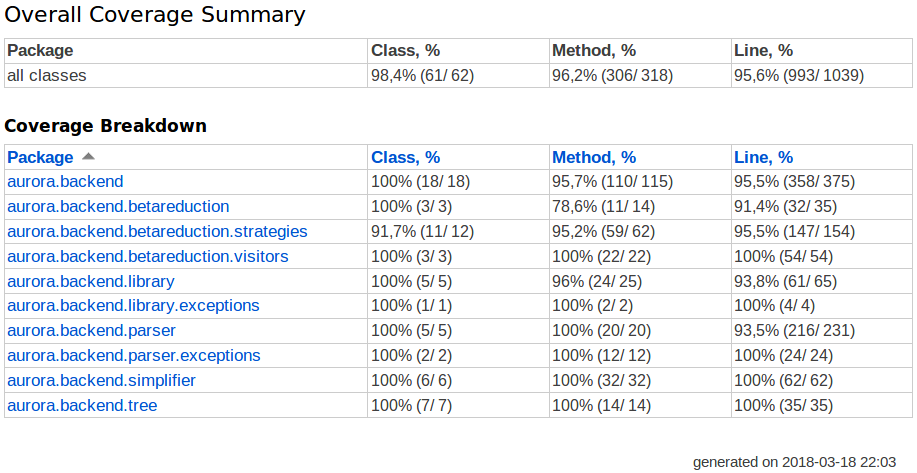
\includegraphics[scale = 0.55]{images/backend.png}
	\end{figure}
	
	Die Zeilenüberdeckung des Backends ist mit diesen zwei Problemfällen bei nur 96\% 
	
	
	Die Überdeckung des Frontends und des Presenter konnte nicht bestimmt werden. 
	Für eine bessere Einschätzung gibt es folgende Werte:
	Die Tests für Frontend und Presenter bestehen aus \textasciitilde 1000 Zeilen Code.
	
	
\end{document}
